 \section{Experiment 2}
 In this experiment we would like to examine the effect of grid resolution by looking at the total displacement per grid node and how the area of the beam is conserved. To measure the total displacement per grid node, we will pointwise take each node in the original beam, and compute the norm of the vector to the same node in the displaced beam and then divide by the total number of grid nodes. Summing these displacements will be our total displacement measure. As we increase the grid resolution we would expect the model accuracy to increase, and thus giving us a better approximation to the real solution. However, its hard to say what the 'true' displacement is, and thus we will also measure the area conservation. We will look at the material steel with Young's modulus $69^9$ and Poisson ratio $0.3$. We will keep the force constant at $-10^7$. We define our smallest grid resolution as 12 by 6 and then we multiply these sizes by an increasing scaling factor. The results for total displacement per node and area conservation can be seen in \autoref{measures}.
 \begin{figure}[H]
 	\centering
 	\begin{subfigure}[b]{0.49\linewidth}
 		\centering
 		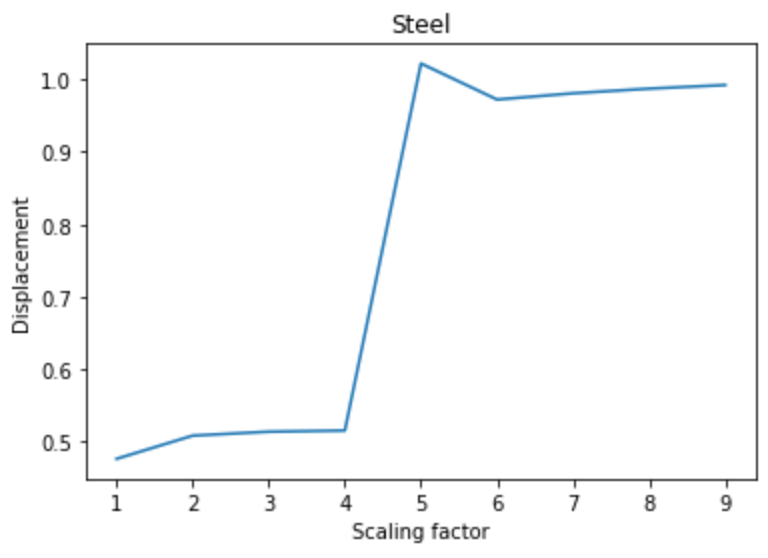
\includegraphics[width=\linewidth]{Materials/Displacement}
 		\caption{Total displacement per node at different grid resolutions.}
 	\end{subfigure}
 	\hfill
 	\begin{subfigure}[b]{0.49\linewidth}
 		\centering
 		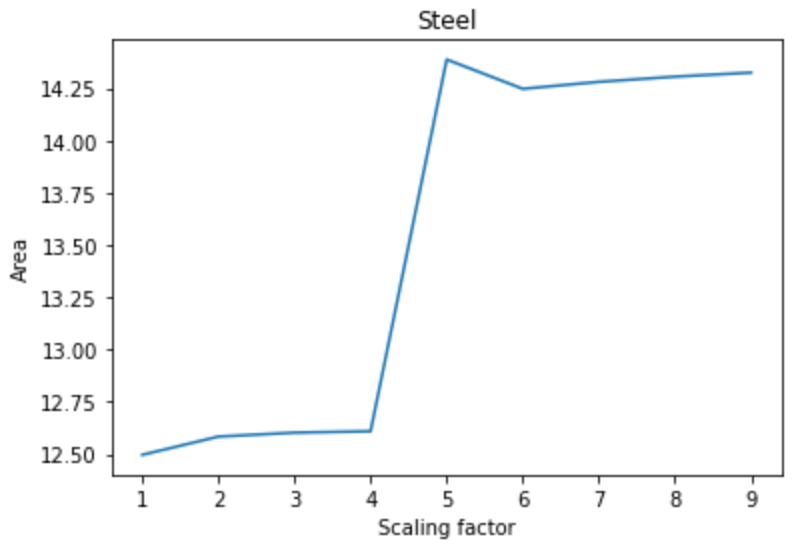
\includegraphics[width=\linewidth]{Materials/Area}
 		\caption{Area of beam at different grid resolutions.}
 	\end{subfigure}
 	\caption{Total displacement per node and area of beam at different grid resolutions at constant force $-10^7$.}
 	\label{measures}
 \end{figure}
We see that the two graphs are very similar which might not be very surprising as the total displacement of the nodes directly influences the area of the beam. We see that the finer grid resolution we use, the more displacement per node we see, and the more area arise. We also see a big change when the grid resolution becomes 60 by 30, where its like the grid is suddenly 'allowed' to bend in its 'desired' way. We can also take a look at how the beams and their deformation looks. This can be seen in \autoref{show}.
 \begin{figure}[H]
	\centering
	\begin{subfigure}[b]{0.49\linewidth}
		\centering
		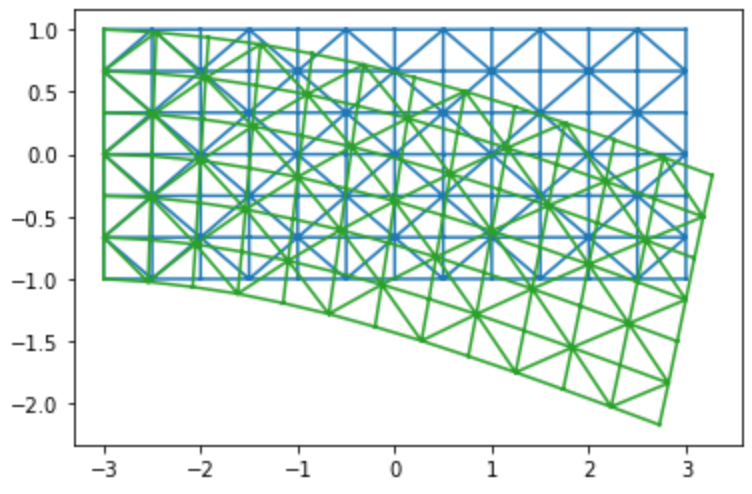
\includegraphics[width=\linewidth]{Materials/Steelviz}
		\caption{Coarse grid.}
	\end{subfigure}
	\hfill
	\begin{subfigure}[b]{0.49\linewidth}
		\centering
		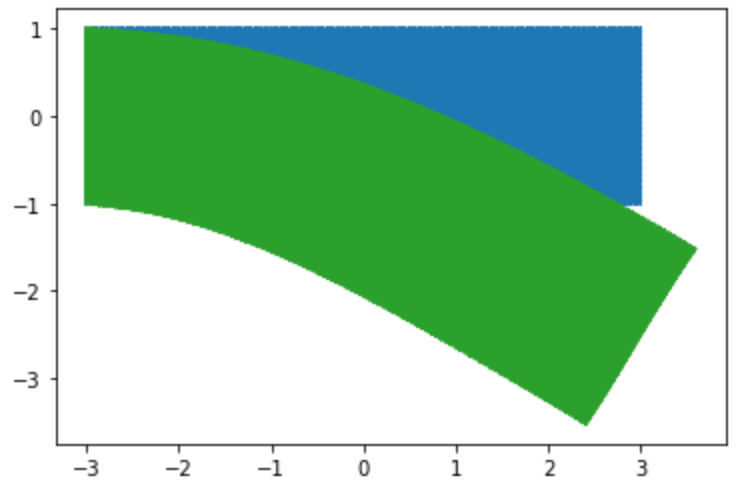
\includegraphics[width=\linewidth]{Materials/Fine}
		\caption{Fine grid.}
	\end{subfigure}
	\caption{Coarse and fine grid resolutions at constant force $-10^7$.}
	\label{show}
\end{figure}
We here clearly see that the displacement is much larger for the finer grid than for the coarse grid as the fine grid has 'sled' all the way down below its original position.

\subsection{Discussion of results}
From \autoref{measures} we clearly see the area and total displacement grows drastically when we increase the grid resolution beyond a factor of 5. The sudden increase could indicate we suddenly have enough nodes for a natural deformation as an increase in grid resolution should improve the model accuracy. However, we would still expect the area to be conserved which it is clearly not. We also see that the total displacement per node graph and the area of the beam graph looks very similar. As the two measures are dependent on each other this might not be very surprising, but this could lead one to think the error in the total displacement is then proportional to the error in increasing area. This could lead to an approximation about how the total displacement per node should look like whereas it would be hard to say anything about on its own.  